\subsection{Title of work and author and advisor(s) names and affiliations}

The title of the poster is ``Harnessing the Power of Many: Extensible Toolkit 
for Scalable Ensemble Applications''. The author presenting the poster will be 
Vivek Balasubramanian, ECE, Rutgers, the State University of New Jersey, under 
the guidance of Dr. Shantenu Jha and Dr. Matteo Turilli, ECE, Rutgers, the State
University of New Jersey.

% Brief description of work being done, including problem being addressed and 
% the research methodology being used
\subsection{Description of research work}

Many scientific problems solved on HPCs consist of applications that rely on the
collective output of multiple tasks as opposed to a single large task. The 
individual tasks within a collection might have different levels of coupling
and communication. This is in contrast to traditional parameter sweeps, or 
high-throughput computing (HTC) applications, where the tasks are typically
identical, uncoupled, idempotent and can be executed in any order. We call a
set of such tasks as an ensemble where an application may consist of multiple 
ensembles.

The execution of an ensemble-based application (EBA) on HPC machines presents 
three main challenges: (1) encoding scientific problems into algorithms that are 
amenable to distributed and coordinated solution; (2) sizing, acquiring, and 
managing resources for the execution; and (3) managing the execution of the 
ensemble.

In the absence of generic solutions to these challenges, we designed and 
implemented the Ensemble Toolkit (EnTK). EnTK addresses these challenges by 
decoupling the description of ensemble-based applications from their execution.
Engineered for scale and diversity, EnTK adheres to the building blocks 
approach~\cite{review_bb_2016} and thus supports coupling with existing runtime 
systems. In addition to extensibility, EnTK enables composability by providing 
components specifically to create EBAs
% . These features enable EnTK to overcome 
% flexibility constraints of monolithic workflow systems, 
and support a wide range of applications.

% EnTK is engineered for scale and diversity of computing platforms and runtime 
% systems. EnTK addresses these challenges by decoupling the description of 
% ensemble-based applications from their execution into three separate orders of 
% concern: specification of task and resource requirements; resource selection and
% acquisition; and task execution management.

\subsection{Abstract of results to be presented in poster}

We present three sets of results in the poster. We first present the performance
benchmark of an EnTK prototype that provides a reference hardware configuration 
to support execution of up to $O(10^6)$ tasks. In the second set of results, we
present the weak and strong scaling behavior of EnTK. Lastly, we implement and 
execute at scale our two use cases, seismic inversion and adaptive analog 
algorithm (AUA).

We prototyped EnTK instantiating multiple producers and consumers of tasks.
The producers push into RabbitMQ queues and consumers pull from these queues.
With a total of $10^6$ tasks, we benchmark the prototype to observe the total
execution time, base and peak memory consumption as a function of the number of
producers, consumers and queues.
% \begin{figure} 
% 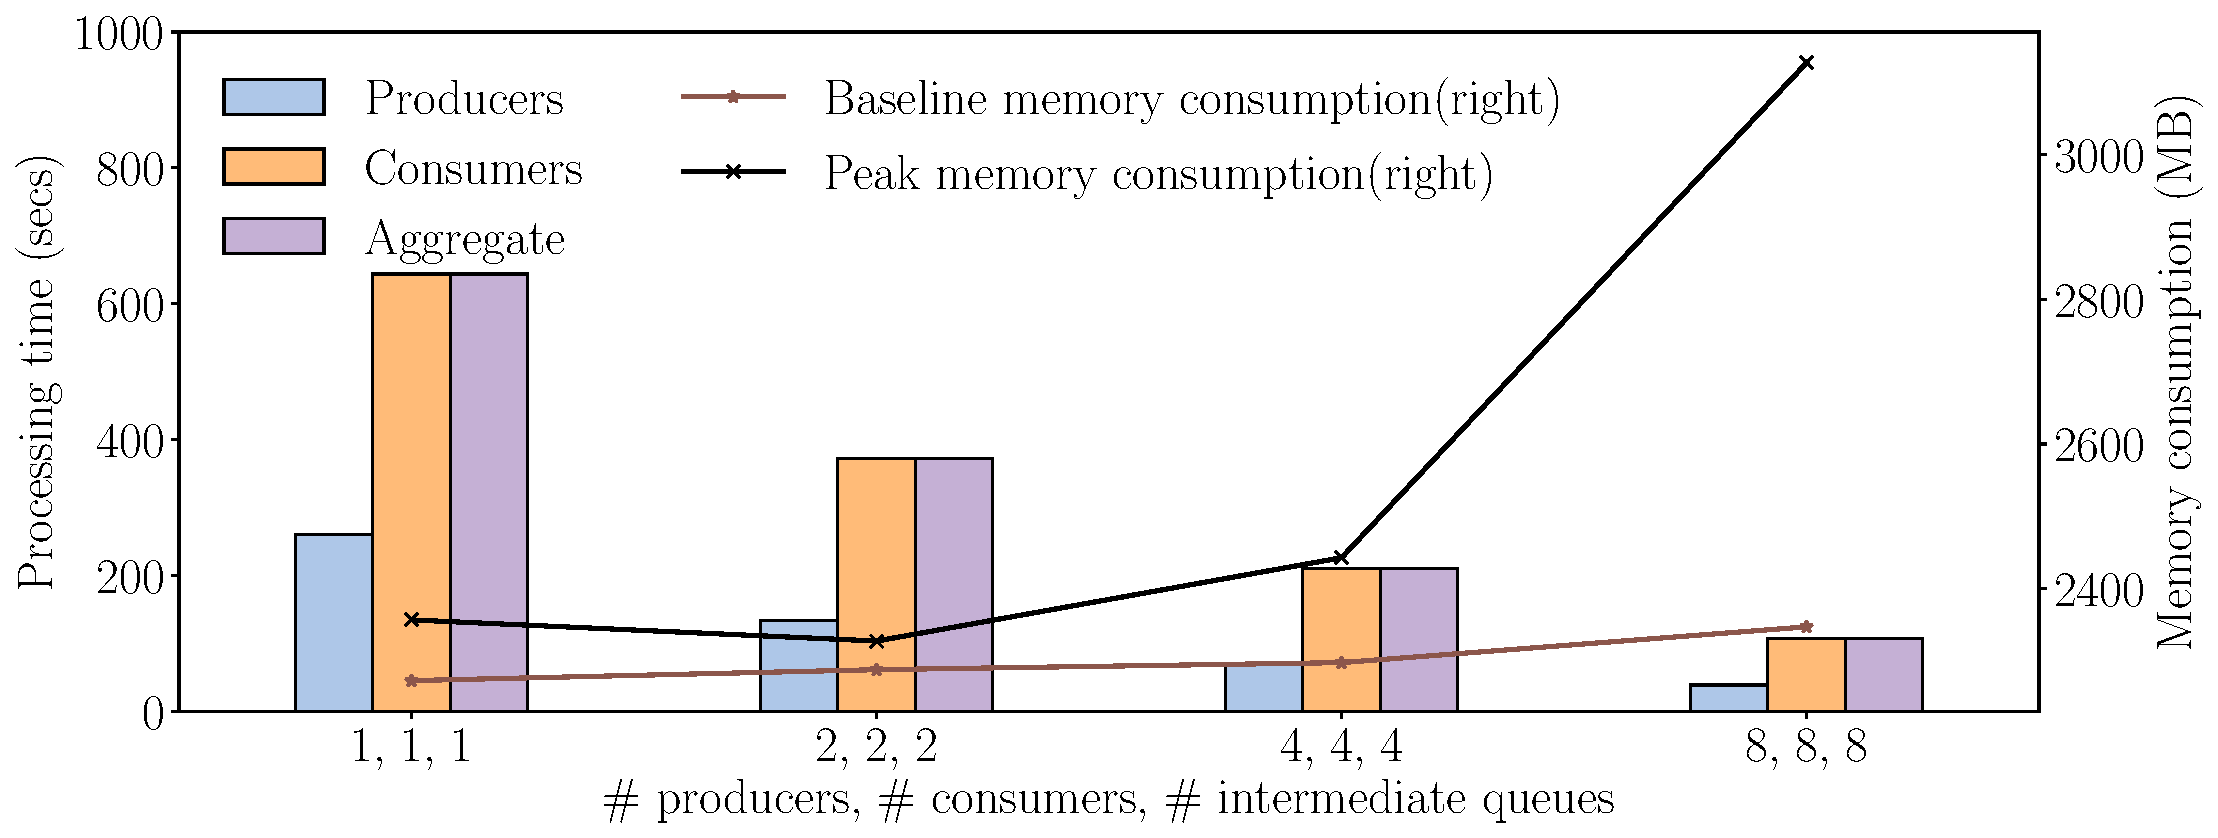
\includegraphics[width=0.48\textwidth]{figs/prototype.pdf}
% \caption{Execution time and memory consumed by EnTK prototype with multiple 
% producers and consumers and $O(10^6)$ tasks}\label{fig:prototype}
% \end{figure}
% In Figure~\ref{fig:prototype}, 
We showed that the execution duration decreases linearly at the cost of 
increased memory usage. We also gather from the benchmark that EnTK can be 
tuned, by varying the number of producers, consumers and queues, depending on 
the resource and application requirements.


Next we present experiments to characterize weak and strong scalability of EnTK.
% Weak scaling experiments describe the performance of EnTK when supporting 
% varying levels of concurrency; Strong scaling experiments describe the 
% performance of EnTK when executing a workload larger than the amount of 
% available resources. 
We focus only on the Task Execution Time, EnTK Management Overhead and Data 
Staging Duration. The remaining durations are a function of the Python language 
or the underlying RTS. Enhancements to these will directly reflect improvements 
in these durations and thus we consider them out of scope.

In the case of weak scaling, we run four applications each with 512, 1024, 2048 
and 4096 tasks and number of cores proportional to the number of tasks. In the 
case of strong scaling, we run three applications each with 8192 tasks and 
1024, 2048 and 4096 cores. Each task, configured to run on 1 core for 
\(\approx\)600 seconds, executes a Gromacs simulation where 550KB of input data 
is moved.
\begin{figure}
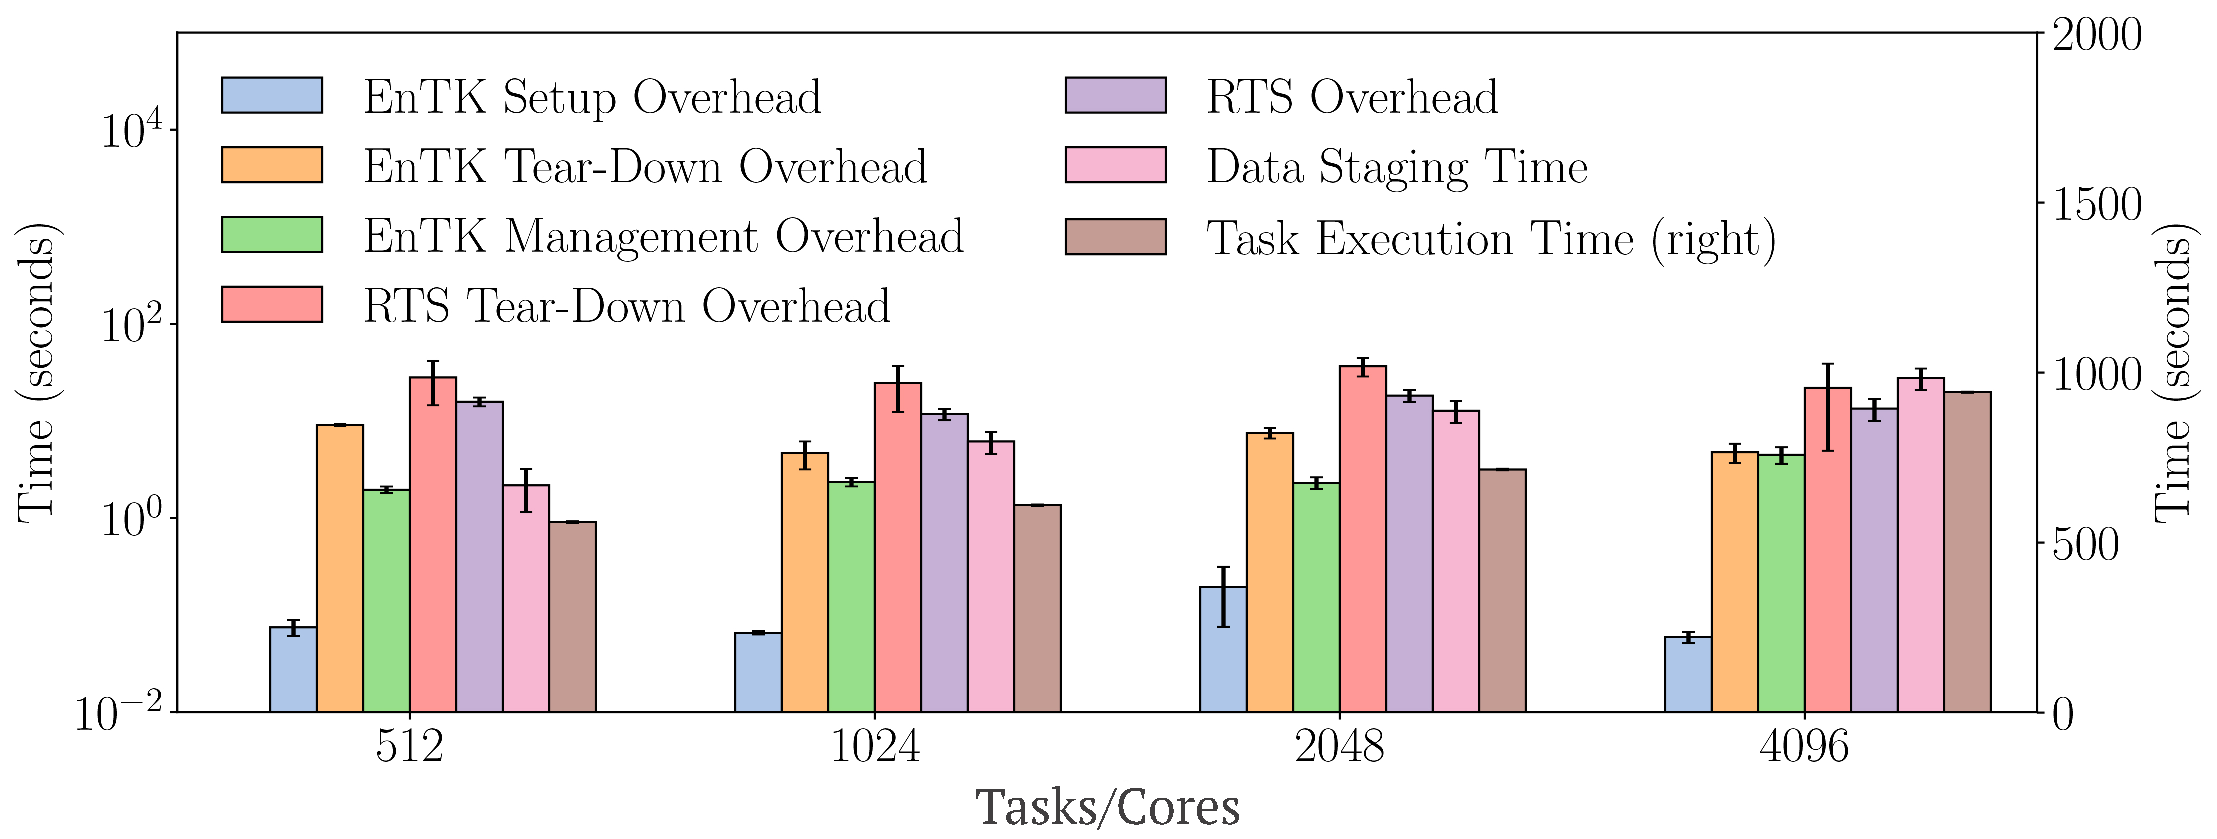
\includegraphics[width=0.48\textwidth]{figs/weak_scaling_titan_orte_reduced.pdf}
\caption{Weak scalability on Titan: 512, 1,024, 2,048, and 4,096
1-core tasks executed on the same amount of cores}\label{fig:weak_scaling}
\end{figure}

In Figure~\ref{fig:weak_scaling}, the Task Execution Time increases even though
there are sufficient resources to run all the tasks. We attribute this to the
limitations in the current implementation of the RTS and the ORTE distributed 
virtual machine. EnTK Management Overhead remains constant up to 2048,
above which the number of tasks strain the resources leading to an increase in
the overhead. The Data Staging Duration increases since the total amount of 
data increases with increase in the number of tasks.

\begin{figure}
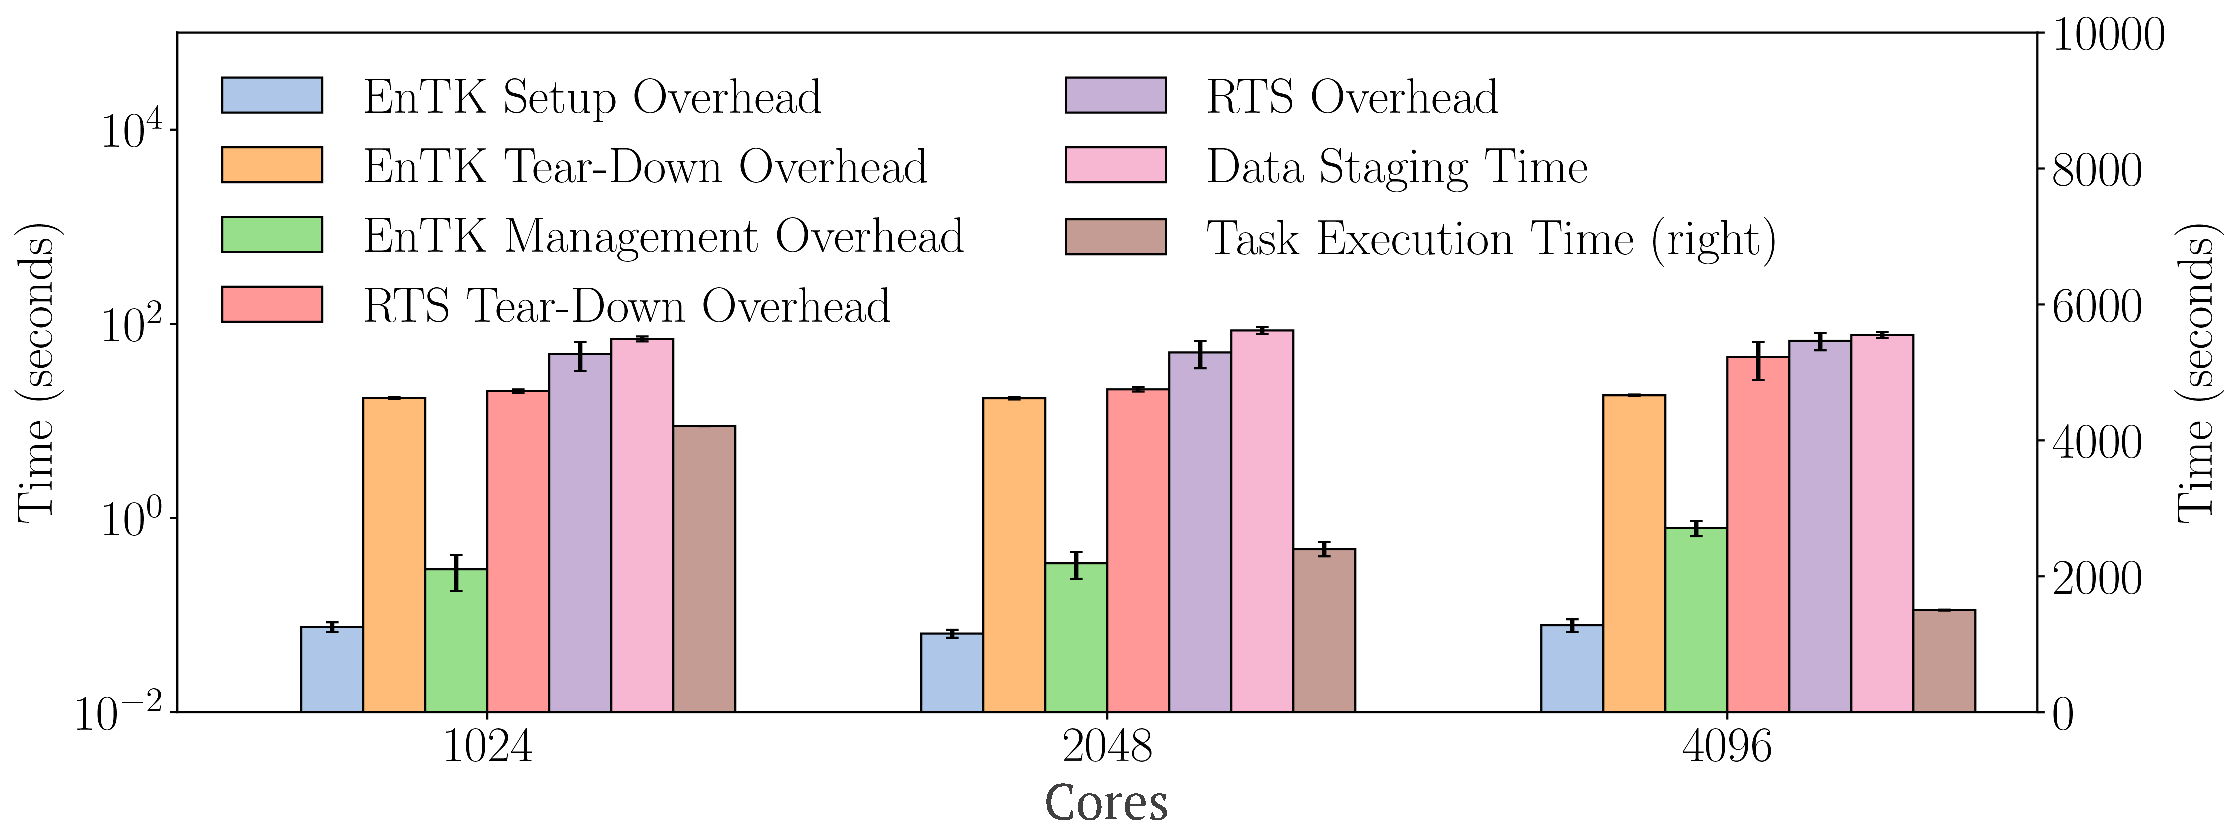
\includegraphics[width=0.48\textwidth]{figs/strong_scaling_titan_orte.pdf}
\caption{Strong scalability on Titan: 8192 1-core tasks executed on 1024, 
2048 and 4096 cores}\label{fig:strong_scaling}
\end{figure}

In Figure~\ref{fig:strong_scaling}, the Task Execution Time reduces linearly 
with an increase in the number of available cores due to a decrease in the 
number of tasks that are executed sequentially. EnTK Management Overhead 
remains constant at \(\approx\)8 seconds and Data Staging Duration remains 
constant at \(\approx\)90 seconds since the total number of tasks remains
constant and thus the total data staged is also constant.

We use EnTK to encode the forward simulations of the seismic inversion workflow.
We show EnTK's capability to handle a failure rate of \(\approx\)79\% observed
when executing $2^5$ simulations concurrently utilizing 75\% of ORNL Titan. We
also implemented the Adaptive Unstructured Analog algorithm at scale using EnTK 
to predict weather forecasts. We observed predictions to converge faster in the 
AUA algorithm than in the random selection.

% We use EnTK to implement the AUA algorithm to iteratively and dynamically 
% identify locations of the analogs. We will also present our results of this
% implementation comparing it with the status quo method, i.e. random selection of
% locations, and observe the speedup of the proposed algorithm.

% \begin{figure} 
% 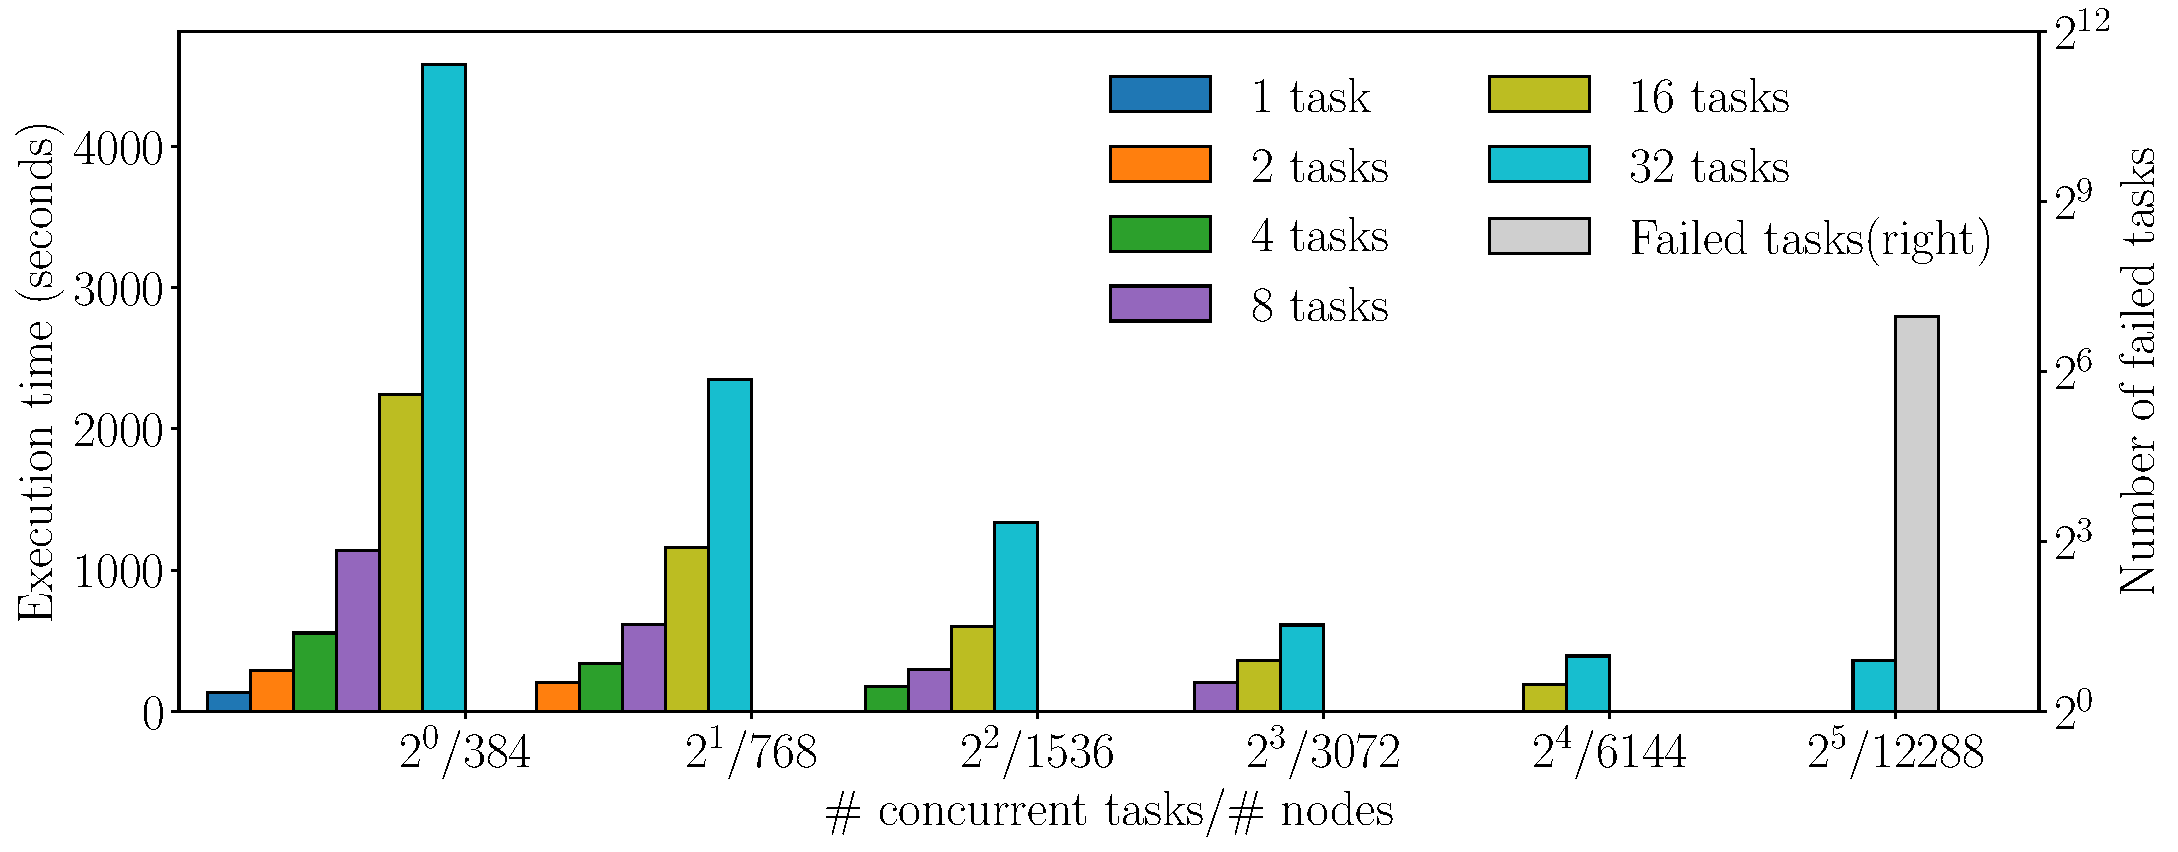
\includegraphics[width=0.48\textwidth]{figs/specfem_exec_time_varying_concurrency_titan.pdf}
% \caption{Task  Execution  Time  of  forward  simulations  using EnTK at various 
% values of concurrency}\label{fig:specfem}
% \end{figure}

% In Figure~\ref{fig:specfem}, we run six applications with 1 pipeline, 1 stage 
% per pipeline and 1, 2, 4, 8, 16 and 32 tasks per stage. Each of the applications
% is run at different levels of concurrency. We observe that for constant
% concurrency, the execution time increases linearly with increase in the number 
% of tasks and the execution time reduces linearly when increasing the 
% concurrency. The increase in the execution time can be explained in terms of the
% number of sequential set of tasks executed which increases in the former and
% decreases in the latter. We also observe that reducing concurrency eliminates 
% failures: we encountered no failures in executions with up to $2^4$ concurrent 
% tasks and 6,144 nodes. At $2^5$ concurrent tasks and 12,288 nodes, 157 tasks 
% failed. We attribute this to the HPC system's limitations to reliably support 
% concurrent execution of simulations which not only use 90\% of the systems 
% compute nodes but also write $2^{20}$ bytes of data per simulation to disk. 
% EnTK automatically submits a failed tasks and as a result we observed a Task 
% Execution Time of \(\approx\)360 seconds, a duration similar to the concurrent
% execution of $2^4$ tasks.


% We use EnTK to implement the AUA algorithm to iteratively and dynamically 
% identify locations of the analogs. We will also present our results of this
% implementation comparing it with the status quo method, i.e. random selection of
% locations, and observe the speedup of the proposed algorithm.

% \begin{figure} 
% 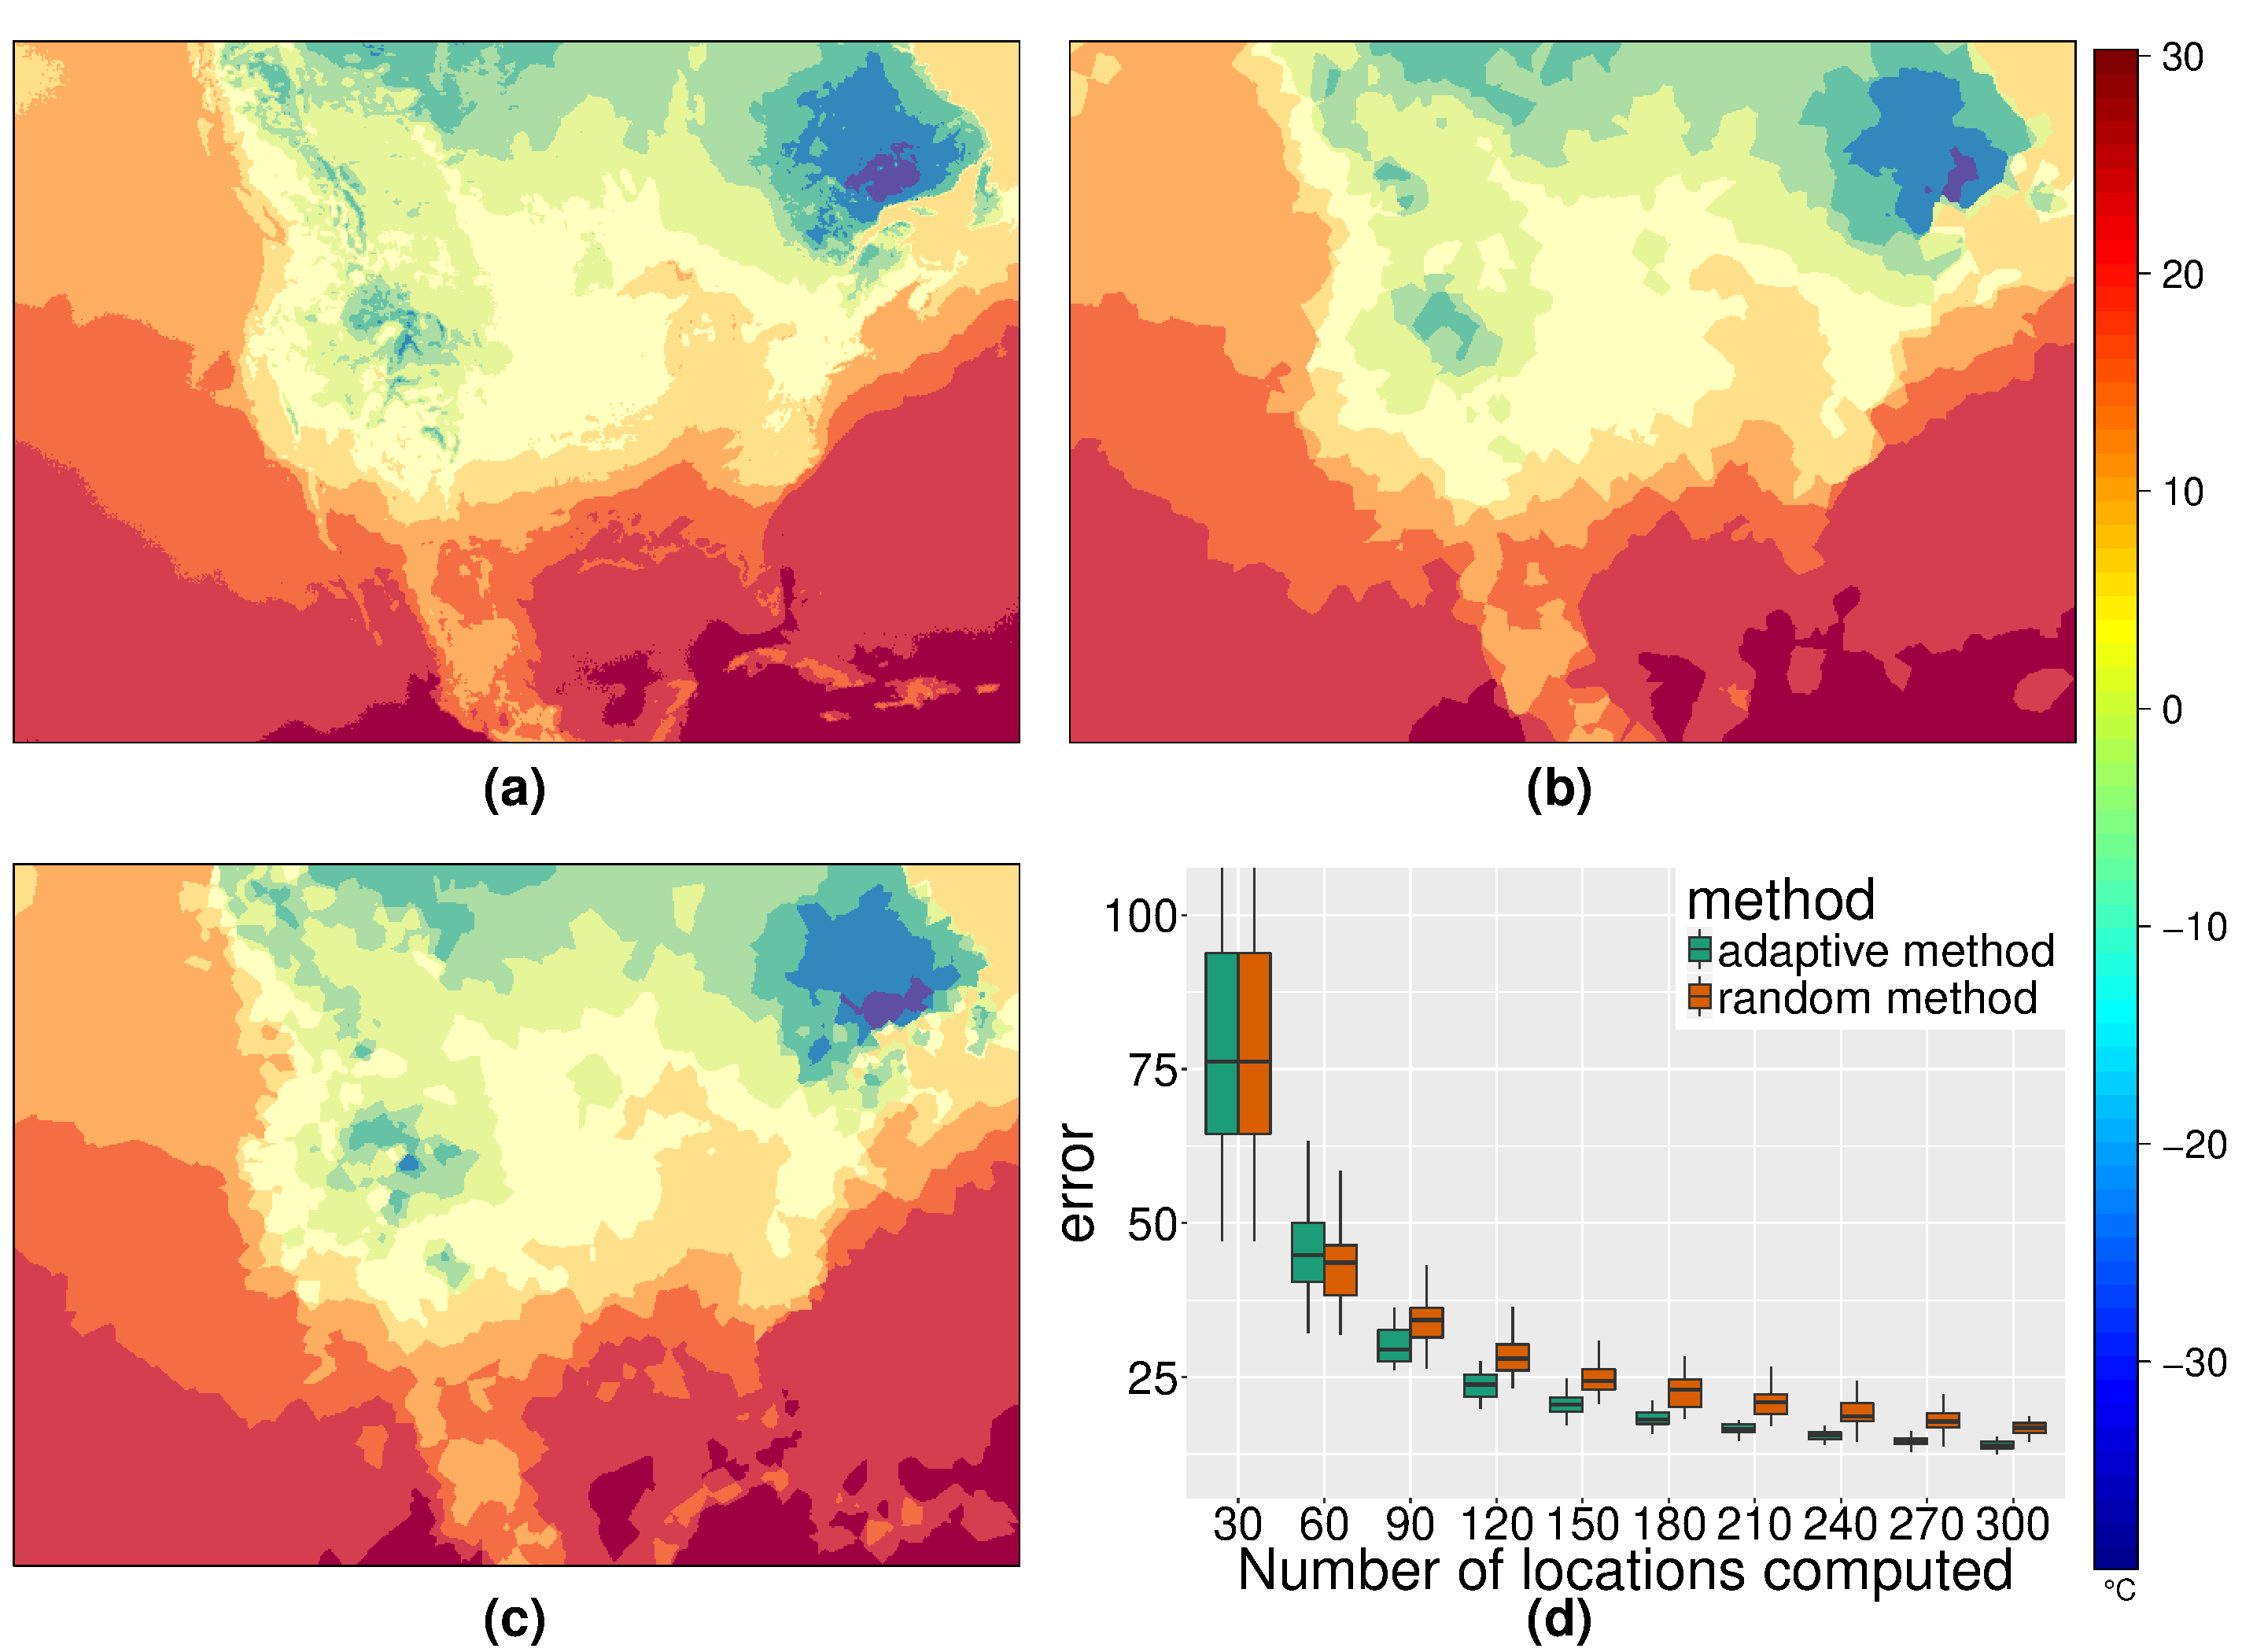
\includegraphics[width=0.48\textwidth]{figs/EX_PSU_error_plot_2x2.pdf}
% \caption{Predictions from random and adaptive methods. (a) theoretical true 
% value, (b) the interpolated map from 1,800 randomly picked locations, (c) the 
% interpolated map from 1,800 locations identified using AUA, (d) box plots of the
% errors for both implementations}\label{fig:anen}
% \end{figure}

% Figure~\ref{fig:anen} shows the prediction maps and errors obtained from the two
% implementations. The AUA algorithm generates a map (c) with certain 
% areas that have a better representation of the analysis than the map generated 
% by a random selection of pixels (b). Box plot (d) shows that the error converges 
% faster in the AUA algorithm than in the random selection.